\subsection{Industry Progress}

The blockchain industry has seen a tremendous pace of development over the past few years, exploring applications and opportunities built on these systems. With this rapid expansion, the industry faces a major technical challenge in improving processing capacity of the blockchain to achieve higher throughput while still maintaining its security. Currently, some very prominent teams have made great progress to achieve this, such as PSE \cite{website:pse}, Matter Labs \cite{website:matter-labs}, Polygon Hermez \cite{website:hermez}, StarkWare \cite{website:starkware}, Risc0 \cite{website:risc0} and Scroll \cite{website:scroll}.

We are able to divide the above mentioned projects into three different levels based on differences in their compatibility with EVM: Consensus-level, Bytecode-level, and Language-level.

First up is PSE, that has a Consensus-level compatibility with EVM, meaning it is fully compatible with EVM. The ZK constraints are consistent with the current behaviour of EVM, this includes the update of the state root, which is advantageous in that you only need to design the circuit to constrain all the rows of EVM. Secondly, Scroll and Polygon has a Bytecode-level compatibility with EVM, which directly interprets the bytecode of EVM, whilst using a different account model to increase ZK efficiency, resulting in different state roots. The advantage of this is that the compatibility with EVM is still guaranteed and the proof efficiency of state root is improved. Due to the introduction of different account models, additional changes at EVM level are required compared to a Consensus-level scheme. Last up is Language-level compatibility, utilized by projects such as StarkWare, Matter Labs and Risc0. They define a ZK-friendly VM, which includes a custom instruction set, custom memory model and so on. They convert Solidity (or Yul) into custom VM-supported instructions through a compiler. The advantage of this solution is achieving that allows for deploying most contracts directly without modification and at the same time providing the highest ZK efficiency in its smaller execution traces and simple state transition constraints. However, trade-offs lie in huge workloads involving constraint design, VM design and compiler design, amongst others. Following we will briefly introduce the general framework of the three mentioned schemes.

\subsubsection{Consensus-level Compatibility}

The main advantage of this scheme is that it maintains full compatibility to the current behaviour of EVM. All behaviors of EVM are constrained by circuits, including but not limited to memory access, instruction execution, and world state updates. Execution traces are generated by EVM Runner, then it is generating a proof that EVM produces combined with its corresponding ZK constraint. The framework of this scheme is shown in Figure \ref{fig:zkevm-architecture-consensus-level}.
\begin{figure}[!ht]
    \centering
    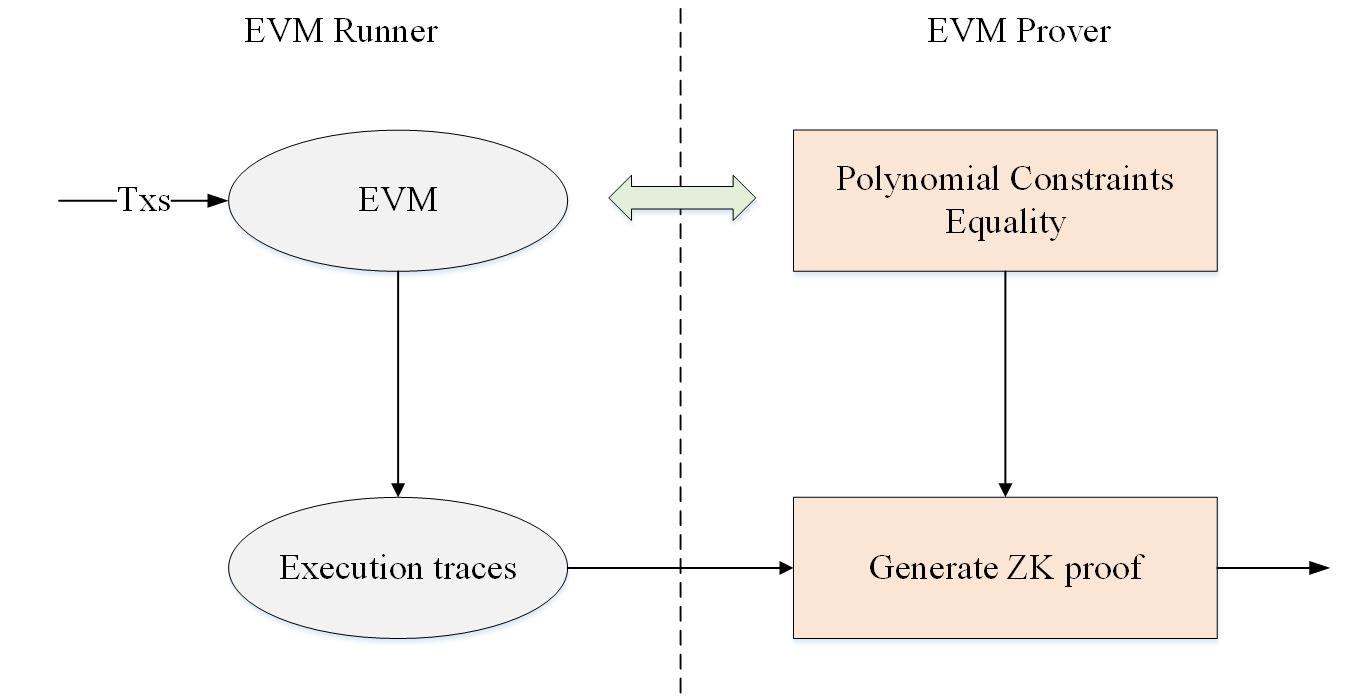
\includegraphics[width=0.8\textwidth]{zkevm-architecture-consensus-level.jpg}
    \caption{ZKEVM architecture based on Consensus-level}
    \label{fig:zkevm-architecture-consensus-level}
\end{figure}

The main workload of this scheme lies in the design of ZK constraints which does not require any modifications to EVM. Which is advantageous, but it is also disadvantageous because there are ZK-unfriendly operations in EVM that also must be proven by ZK-constraints, which makes the overall ZK efficiency low.

\subsubsection{Bytecode-level Compatibility}

Intuitively you may assume that the feature of this scheme is that it can process all the instructions of EVM on Bytecode-level (That the bytecodes of a Solidity contract can be directly used as input), however, other parts than the instructions can be different, such as getting a different state root and using a different hash algorithm. The framework of the scheme is shown in Figure \ref{fig:zkevm-architecture-bytecode-level}.
\begin{figure}[!ht]
    \centering
    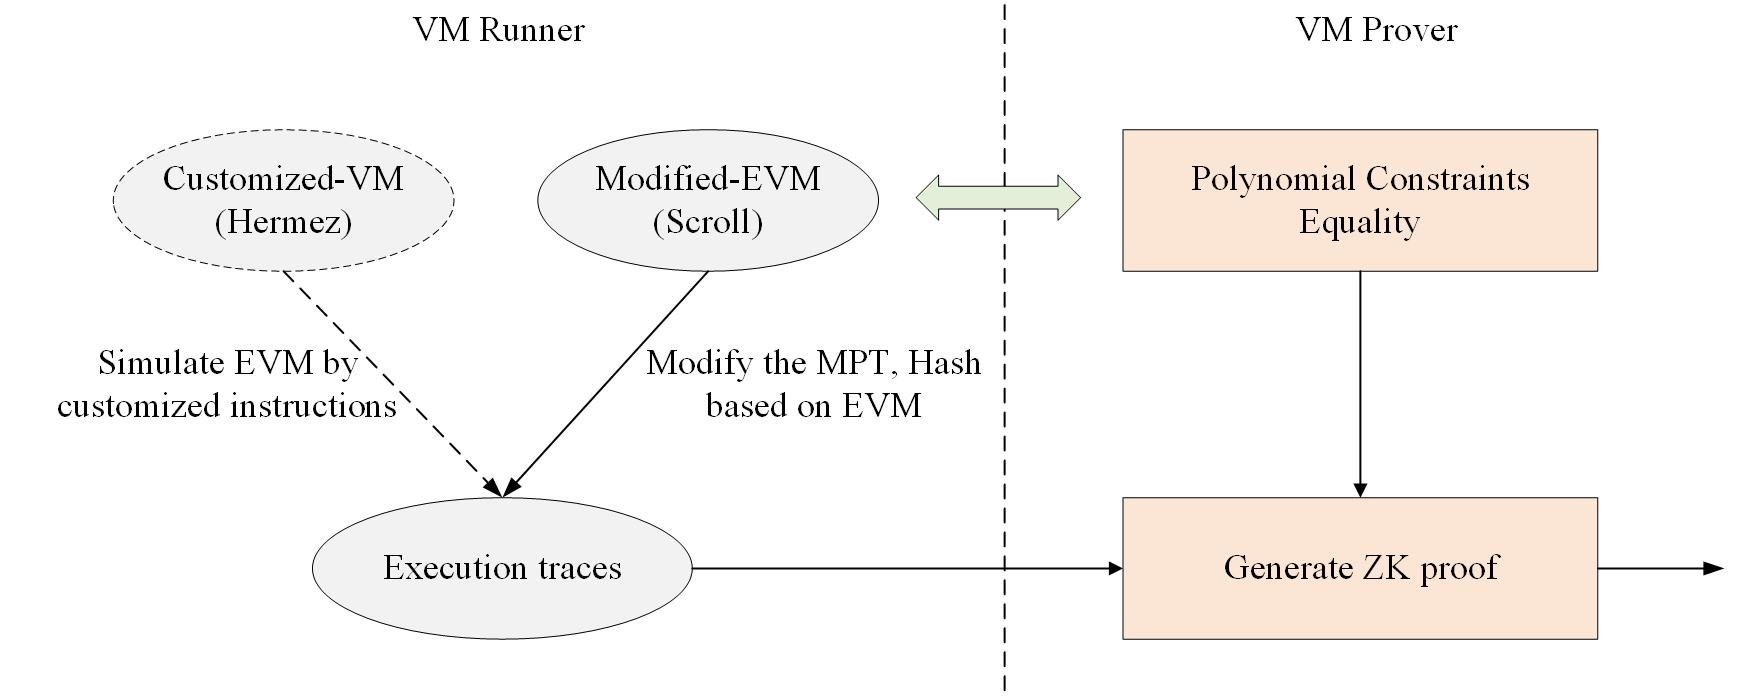
\includegraphics[width=0.8\textwidth]{zkevm-architecture-bytecode-level.jpg}
    \caption{ZKEVM architecture based on Bytecode-level}
    \label{fig:zkevm-architecture-bytecode-level}
\end{figure}

As you can tell by this scheme it requires designing or modifying the VM in addition to designing ZK constraints. As an example, Scroll may only need to make corresponding modifications based on the Ethereum client, but Hermez is slightly more complicated due to them customizing a VM. Compared with the Consensus-level ZKEVM scheme, the ZK efficiency of this scheme is slightly better.

\subsubsection{Language-level Compatibility}

Compared to previous two schemes, Language-level compatibility is the weakest. It does not have to be 100\% compatible with EVM, which means that simple modifications to some contracts could result in it needing a lot of support. However, the overall scheme has a ZK-friendly design, e.g, the memory model, instruction set, account model and so on, hence it has a better ZK efficiency. The framework of this scheme is shown in Figure \ref{fig:zkevm-architecture-language-level}.
\begin{figure}[!ht]
    \centering
    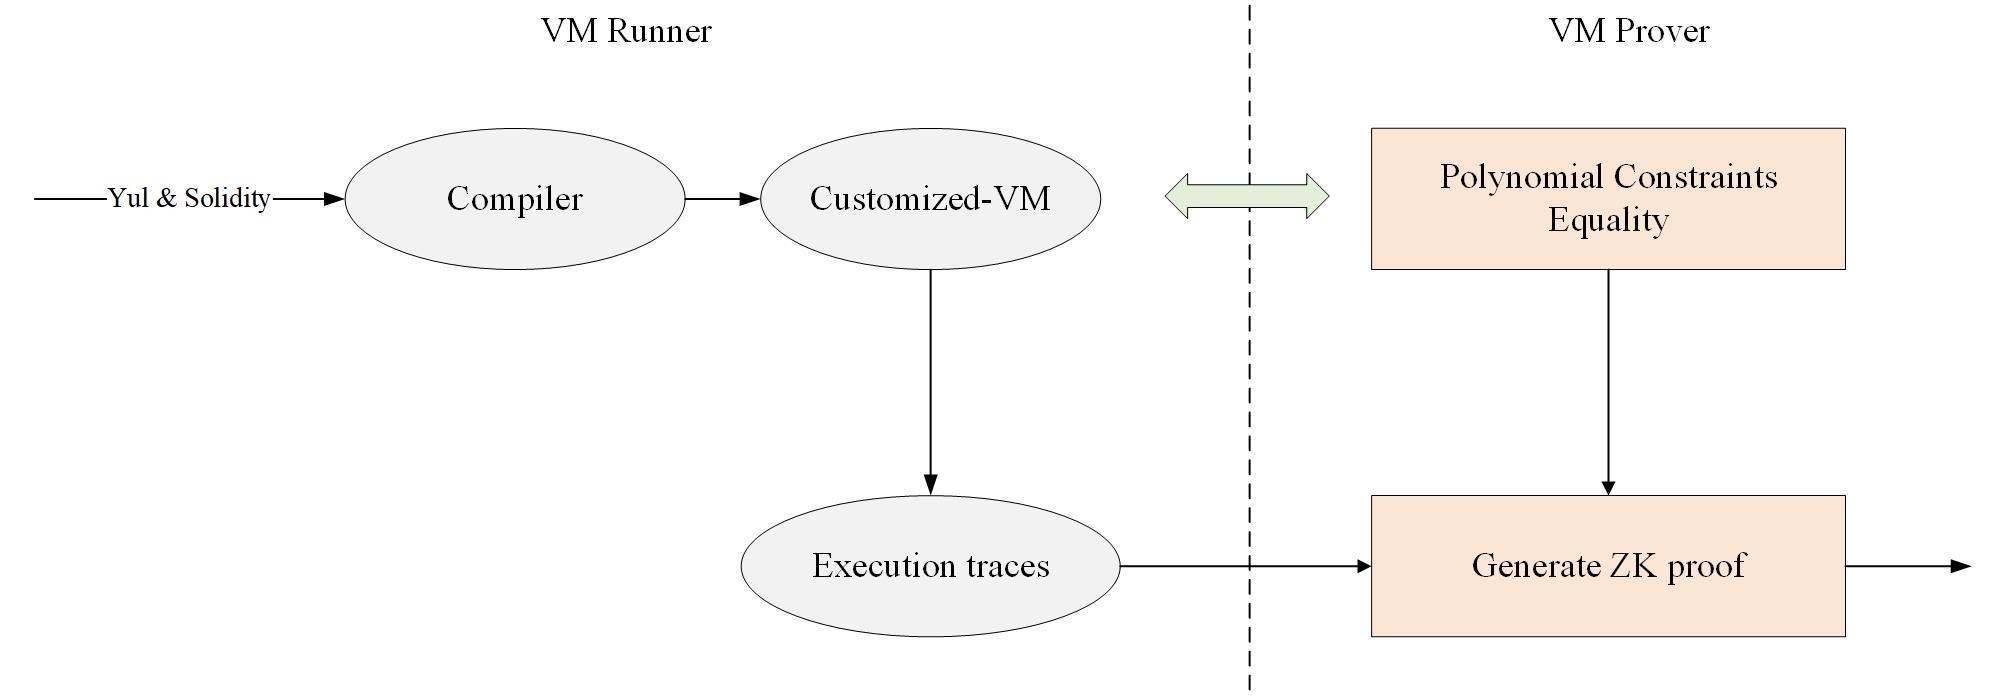
\includegraphics[width=0.8\textwidth]{zkevm-architecture-language-level.jpg}
    \caption{ZKEVM architecture based on Language-level}
    \label{fig:zkevm-architecture-language-level}
\end{figure}

Out of all the schemes this has the highest workload, involving the compiler, VM \& constraint design and so on. However, it is also achieving the best ZK efficiency. An example would be StarkWare's Cairo VM, which has a surprisingly good performance in terms of capacity expansion. StarkWare team has come quite far with the Cairo design in terms of being ZK-friendly since the inception of teams pursuing developing a ZKEVM solution.
